\section{Embedded Linux application development}

\begin{frame}
  \frametitle{Contents}
  \begin{itemize}
  \item Application development
    \begin{itemize}
    \item Developing applications on embedded Linux
    \item Building your applications
    \end{itemize}
  \item Source management
    \begin{itemize}
    \item Integrated development environments (IDEs)
    \item Version control systems
    \end{itemize}
  \item Debugging and analysis tools
    \begin{itemize}
    \item Debuggers
    \item Memory checkers
    \item System analysis
    \end{itemize}
  \item Development environments
    \begin{itemize}
    \item Developing on Windows
    \end{itemize}
  \end{itemize}
\end{frame}

\subsection{Developing applications on embedded Linux}

\begin{frame}
  \frametitle{Application development}
  \begin{itemize}
  \item An embedded Linux system is just a normal Linux system, with
    usually a smaller selection of components
  \item In terms of application development, developing on embedded
    Linux is exactly the same as developing on a desktop Linux system
  \item All existing skills can be re-used, without any particular
    adaptation
  \item All existing libraries, either third-party or in-house, can be
    integrated into the embedded Linux system
    \begin{itemize}
    \item Taking into account, of course, the limitation of the
      embedded systems in terms of performance, storage and memory
    \end{itemize}
  \end{itemize}
\end{frame}

\begin{frame}
  \frametitle{Programming language}
  \begin{itemize}
  \item The default programming language for system-level application
    in Linux is usually C
    \begin{itemize}
    \item The C library is already present on your system, nothing to
      add
    \end{itemize}
  \item C++ can be used for larger applications
    \begin{itemize}
    \item The C++ library must be added to the system
    \item Some libraries, including Qt, are developed in C++ so they
      need the C++ library on the system anyway
    \end{itemize}
  \item Scripting languages can also be useful for quick application
    development, web applications or scripts
    \begin{itemize}
    \item But they require an interpreter on the embedded system and
      have usually higher memory consumption and slightly lower
      performances
    \end{itemize}
  \item Languages: Python, Perl, Lua, Ada, Fortran, etc.
  \end{itemize}
\end{frame}

\begin{frame}
  \frametitle{C library or higher-level libraries?}
  \begin{itemize}
  \item For many applications, the C library already provides a
    relatively large set of features
    \begin{itemize}
    \item file and device I/O, networking, threads and
      synchronization, inter-process communication
    \item Thoroughly described in the glibc manual, or in any {\em
        Linux system programming} book
    \item However, the API carries a lot of history and is not
      necessarily easy to grasp for new comers
    \end{itemize}
  \item Therefore, using a higher level framework, such as Qt or the
    Gtk stack, might be a good idea
    \begin{itemize}
    \item These frameworks are not only graphical libraries, their
      core is separate from the graphical part
    \item But of course, these libraries have some memory and storage
      footprint, in the order of a few megabytes
    \end{itemize}
  \end{itemize}
\end{frame}

\begin{frame}
  \frametitle{Building your applications}
  \begin{itemize}
  \item For simple applications that do not need to be really portable
    or provide compile-time configuration options, a simple Makefile
    will be sufficient
  \item For more complicated applications, or if you want to be able
    to run your application on a desktop Linux PC and on the target
    device, using a build system is recommended
    \begin{itemize}
    \item Look at the {\em autotools} (ancient, complicated but very
      widely used) or {\em CMake} (modern, simpler, smaller but
      growing user base)
    \end{itemize}
  \item The QT library is a special case, since it comes with its own
    build system for applications, called qmake
  \end{itemize}
\end{frame}

\begin{frame}[fragile]
  \frametitle{Simple Makefile (1)}
  \begin{itemize}
  \item Case of an application that only uses the C library, contains two source
    files and generates a single binary
  \end{itemize}
\begin{block}{}
\begin{verbatim}
CROSS_COMPILE?=arm-linux-
CC=$(CROSS_COMPILE)gcc
OBJS=foo.o bar.o

all: foobar

foobar: $(OBJS)
        $(CC) -o $@ $^

clean:
        $(RM) -f foobar $(OBJS)
\end{verbatim}
\end{block}
\end{frame}

\begin{frame}[fragile]
  \frametitle{Simple Makefile (2)}
\begin{itemize}
\item Case of an application that uses the Glib and the GPS libraries
\end{itemize}
\small
\begin{block}{}
\begin{verbatim}
CROSS_COMPILE?=arm-linux-
LIBS=libgps glib-2.0
OBJS=foo.o bar.o

CC=$(CROSS_COMPILE)gcc
CFLAGS=$(shell pkg-config --cflags $(LIBS))
LDFLAGS=$(shell pkg-config --libs $(LIBS))

all: foobar

foobar: $(OBJS)
        $(CC) -o $@ $^ $(LDFLAGS)

clean:
        $(RM) -f foobar $(OBJS)
\end{verbatim}
\end{block}
\end{frame}

\subsection[Source management \& IDEs]{Source management \& Integrated
  Development Environments (IDE)}

\begin{frame}
  \frametitle{Source browsers}
  \begin{itemize}
  \item {\bf LXR: Linux Cross Reference}\\
    Allows to browse code through a web browser.
  \item {\bf cscope}\\
    Console mode source browsing tool.\\
    Integrates with editors like vi and Emacs.
\end{itemize}
See our Linux kernel and driver development training materials\\
(\url{http://free-electrons.com/docs/kernel}) for more details.
\end{frame}

\begin{frame}
  \frametitle{KDevelop}
  \begin{columns}[T]
    \column{0.8\textwidth}
    \url{http://kdevelop.org}
    \begin{itemize}
    \item A full featured IDE!
    \item License: GPL
    \item Supports many languages: Ada, C, C++, Database, Java, Perl,
      PHP, Python, Ruby, Shell
    \item Supports many kinds of projects: KDE, but also GTK, Gnome,
      kernel drivers, embedded (Opie)...
    \item Many features: editor, syntax highlighting, code completion,
      compiler interface, debugger interface, file manager, class
      browser...
    \end{itemize}
    Nice overview: \url{http://en.wikipedia.org/wiki/Kdevelop}
    \column{0.2\textwidth}
    
\includegraphics[width=\textwidth]{slides/sysdev-application-development/kdevelop.png}
  \end{columns}
\end{frame}

\begin{frame}
  \frametitle{KDevelop screenshot}
  \begin{center}
    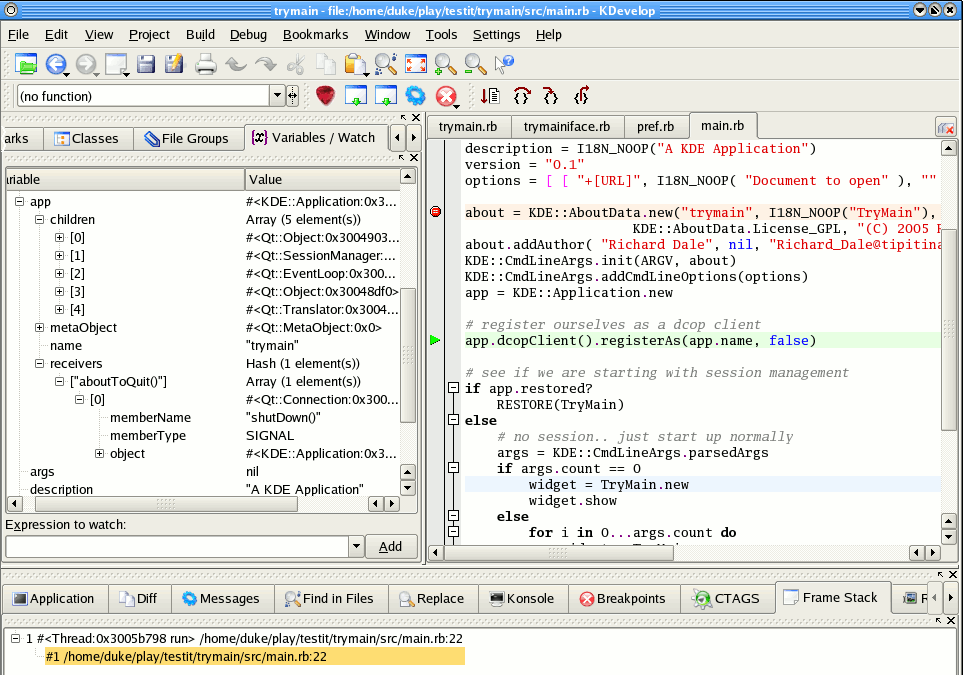
\includegraphics[width=0.9\textwidth]{slides/sysdev-application-development/kdevelop-screenshot.png}\\
    Ruby debugger
  \end{center}
\end{frame}

\begin{frame}
  \frametitle{Eclipse (1)}
  \begin{columns}[T]
    \column{0.8\textwidth}
    \url{http://www.eclipse.org/}
    \begin{itemize}
    \item An extensible, plug-in based software development kit,
      typically used for creating IDEs.
    \item Supported by the Eclipse foundation, a non-profit consortium
      of major software industry vendors (IBM, Intel, Borland, Nokia,
      Wind River, Zend, Computer Associates...).
    \item Free Software license (Eclipse Public License). Incompatible
      with the GPL.
    \item Supported platforms: GNU/Linux, Unix, Windows
    \end{itemize}
    Extremely popular: created a lot of attraction.
    \column{0.2\textwidth}
    
\includegraphics[width=0.9\textwidth]{slides/sysdev-application-development/eclipse.png}
  \end{columns}
\end{frame}

\begin{frame}
  \frametitle{Eclipse (2)}
  \begin{itemize}
  \item Eclipse is actually a platform composed of many projects:\\
    \url{http://www.eclipse.org/projects/}
    \begin{itemize}
    \item Some projects are dedicated at integrating into Eclipse
      features useful for embedded developers (cross-compilation,
      remote development, remote debugging, etc.)
    \end{itemize}
  \item The platform is used by major embedded Linux software vendors
    for their (proprietary) system development kits: MontaVista
    DevRocket, TimeSys TimeStorm, Wind River Workbench, Sysgo ELinOS.
  \end{itemize}
  Eclipse is a huge project.  It would require an entire training
  session!
\end{frame}

\subsection{Version control systems}

\begin{frame}
  \frametitle{Version control systems}
  Real projects can't do without them
  \begin{itemize}
  \item Allow multiple developers to contribute on the same
    project. Each developer can see the latest changes from the
    others, or choose to stick with older versions of some components.
  \item Allow to keep track of changes, and revert them if needed.
  \item Allow developers to have their own development branch
    (branching)
  \item Supposed to help developers resolving conflicts with different
    branches (merging)
  \end{itemize}
\end{frame}

\begin{frame}
  \frametitle{Traditional version control systems} Rely on a central
  repository. The most popular open-source ones:
  \begin{itemize}
  \item {\bf CVS - Concurrent Versions System}
    \begin{itemize}
    \item Still quite popular in enterprise contexts. Almost no longer
      exists in the open-source community.
    \item Should no longer be used for new projects
    \item
      \url{http://en.wikipedia.org/wiki/Concurrent_Versions_System}
    \end{itemize}
  \item {\bf Subversion}
    \begin{itemize}
    \item Created as a replacement of CVS, removing many of its
      limitations.
    \item Commits on several files, proper renaming support, better
      performances, etc.
    \item The user interface is very similar to CVS
    \item \url{http://en.wikipedia.org/wiki/Subversion_(software)}
    \end{itemize}
  \end{itemize}
\end{frame}

\begin{frame}
  \frametitle{Distributed source control systems (1)}
  No longer have a central repository
  \begin{itemize}
  \item More adapted to the way the Free Software community develops
    software and organizes
  \item Allows each developer to have a full local history of the
    project, to create local branches. Makes each developer's work
    easier.
  \item People get working copies from other people's working copies,
    and exchange changes between themselves. Branching and merging is
    made easier.
  \item Make it easier for new developers to join, making their own
    experiments without having to apply for repository access.
  \end{itemize}
\end{frame}

\begin{frame}
  \frametitle{Distributed source control systems (2)}
  \begin{itemize}
  \item {\bf Git}
    \begin{itemize}
    \item Initially designed and developed by Linus Torvalds for Linux
      kernel development
    \item Extremely popular in the community, and used by more and
      more projects (kernel, U-Boot, Barebox, uClibc, GNOME, X.org,
      etc.)
    \item Outstanding performance, in particular in big projects
    \item \url{http://en.wikipedia.org/wiki/Git_(software)}
    \end{itemize}
  \item {\bf Mercurial}
    \begin{itemize}
    \item Another system, created with the same goals as Git.
    \item Used by some big projects too
    \item \url{http://en.wikipedia.org/wiki/Mercurial}
    \end{itemize}
  \end{itemize}
  \url{http://en.wikipedia.org/wiki/Version_control_systems\#Distributed_revision_control}
\end{frame}

\subsection{Debuggers}

\begin{frame}
  \frametitle{GDB}
  \begin{columns}[T]
    \column{0.8\textwidth}
    The {\bf GNU Project Debugger}\\
    \url{http://www.gnu.org/software/gdb/}
    \begin{itemize}
    \item The debugger on GNU/Linux, available for most embedded
      architectures.
    \item Supported languages: C, C++, Pascal, Objective-C, Fortran,
      Ada...
    \item Console interface (useful for remote debugging).
    \item Graphical front-ends available.
    \item Can be used to control the execution of a program, set
      breakpoints or change internal variables. You can also use it to
      see what a program was doing when it crashed (by loading its
      memory image, dumped into a core file).
    \end{itemize}
    See also \url{http://en.wikipedia.org/wiki/Gdb}
    \column{0.2\textwidth}
    
\includegraphics[width=0.9\textwidth]{slides/sysdev-application-development/gdb.png}
  \end{columns}
\end{frame}

\begin{frame}
  \frametitle{GDB crash course}
  \begin{itemize}
  \item A few useful GDB commands
    \begin{itemize}
    \item \code{break foobar}\\
      puts a breakpoint at the entry of function \code{foobar()}
    \item \code{break foobar.c:42}\\
      puts a breakpoint in \code{foobar.c}, line 42
    \item \code{print var} or \code{print task->files[0].fd}\\
      prints the variable \code{var}, or a more complicated reference. GDB
      can also nicely display structures with all their members
    \item \code{continue}\\
      continue the execution
    \item \code{next}\\
      continue to the next line, stepping over function calls
    \item \code{step}\\
      continue to the next line, entering into subfunctions
    \end{itemize}
  \end{itemize}
\end{frame}

\begin{frame}
  \frametitle{GDB graphical front-ends}
  \begin{itemize}
  \item {\bf DDD} - Data Display Debugger\\
    \url{http://www.gnu.org/software/ddd/}\\
    A popular graphical front-end, with advanced data plotting
    capabilities.
  \item {\bf GDB/Insight}\\
    \url{http://sourceware.org/insight/}\\
    From the GDB maintainers.
  \item {\bf KDbg}\\
    \url{http://www.kdbg.org/}\\
    Another front-end, for the K Display Environment.
  \item Integration with other IDEs: Eclipse, Emacs, KDevelop, etc.\\
  \end{itemize}
\end{frame}

\subsection{Remote debugging}

\begin{frame}
  \frametitle{Remote debugging}
  \begin{itemize}
  \item In a non-embedded environment, debugging takes place using gdb
    or one of its front-end.
  \item gdb has direct access to the binary and libraries compiled
    with debugging symbols.
  \item However, in an embedded context, the target platform
    environment is often too limited to allow direct debugging with
    gdb (2.4 MB on x86).
  \item Remote debugging is preferred
    \begin{itemize}
    \item \code{gdb} is used on the development workstation, offering
      all its features.
    \item \code{gdbserver} is used on the target system (only 100 KB
      on arm).
    \end{itemize}
  \end{itemize}
  \begin{center}
    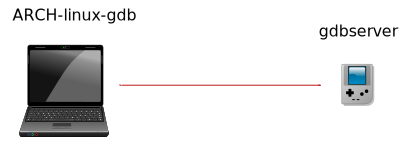
\includegraphics[width=0.5\textwidth]{slides/sysdev-application-development/gdb-vs-gdbserver.pdf}
  \end{center}
\end{frame}

\begin{frame}
  \frametitle{Remote debugging: architecture}
  \begin{center}
    \includegraphics[width=\textwidth]{slides/sysdev-application-development/gdb-vs-gdbserver-architecture.pdf}
  \end{center}
\end{frame}

\begin{frame}
  \frametitle{Remote debugging: usage}
  \begin{itemize}
  \item On the target, run a program through gdbserver.\\
    Program execution will not start immediately.\\
    \code{gdbserver localhost:<port> <executable> <args>}
    \code{gdbserver /dev/ttyS0 <executable> <args>}
  \item Otherwise, attach gdbserver to an already running program:\\
    \code{gdbserver --attach localhost:<port> <pid>}
  \item Then, on the host, run \code{ARCH-linux-gdb} program,\\
    and use the following gdb commands:
    \begin{itemize}
    \item To connect to the target:\\
      \code{gdb> target remote <target>:<port>} (networking)\\
      \code{gdb>  target remote /dev/ttyS0} (serial link)
    \item To tell gdb where shared libraries are:\\
      \code{gdb> set sysroot <library-path>} (without \code{lib/})
    \end{itemize}
  \end{itemize}
\end{frame}

\begin{frame}
  \frametitle{Post mortem analysis}
  \begin{itemize}
  \item When an application crashes due to a {\em segmentation fault}
    and the application was not under control of a debugger, we get no
    information about the crash
  \item Fortunately, Linux can generate a {\em core} file that
    contains the image of the application memory at the moment of the
    crash, and gdb can use this {\em core} file to let us analyze the
    state of the crashed application
  \item On the target
    \begin{itemize}
    \item Use \code{ulimit -c unlimited} to enable the generation of a
      {\em core} file when a crash occurs
    \end{itemize}
  \item On the host
    \begin{itemize}
    \item After the crash, transfer the core file from the target to
      the host, and run
      \code{ARCH-linux-gdb -c core-file application-binary}
    \end{itemize}
  \end{itemize}
\end{frame}

\subsection{Memory checkers}

\begin{frame}
  \frametitle{memcheck}
  \url{http://hald.dnsalias.net/projects/memcheck/}
  \begin{itemize}
  \item GNU GPL tool for dynamic memory checking
  \item Works by replacing glibc's memory management functions by its own.
  \item Supports most useful CPU architectures.
  \end{itemize}
\end{frame}

\begin{frame}
  \frametitle{DUMA}
  Detect Unintended Memory Access\\
  \url{http://duma.sourceforge.net/}
  \begin{itemize}
  \item Fork and replacement for Electric Fence
  \item Stops your program on the exact instruction that overruns or
    underruns a \code{malloc()} memory buffer.
  \item GDB will then display the source-code line that causes the
    bug.
  \item Works by using the virtual-memory hardware to create a
    red-zone at the border of each buffer - touch that, and your
    program stops.
  \item Works on any platform supported by Linux, whatever the CPU
    (provided virtual memory support is available).
  \end{itemize}
\end{frame}

\begin{frame}
  \frametitle{Valgrind (1)}
  \begin{columns}[T]
    \column{0.8\textwidth}
    \url{http://valgrind.org/}
    \begin{itemize}
    \item GNU GPL Software suite for debugging and profiling programs.
    \item Supported platforms: Linux on x86, x86\_64, ppc32, ppc64 and
      arm (armv7 only: Cortex A8, A9 and A5)
    \item Can detect many memory management and threading bugs.
    \item Profiler: provides information helpful to speed up your
      program and reduce its memory usage.
    \item The most popular tool for this usage. Even used by projects
      with hundreds of programmers.
    \end{itemize}
    \column{0.2\textwidth}
    
\includegraphics[width=\textwidth]{slides/sysdev-application-development/valgrind1.png}
  \end{columns}
\end{frame}

\begin{frame}
  \frametitle{Valgrind (2)}
  \begin{columns}[T]
    \column{0.8\textwidth}
    \begin{itemize}
    \item Can be used to run any program, without the need to
      recompile it.
    \item Example usage\\
      \code{Valgrind --leak-check=yes ls -la}
    \item Works by adding its own instrumentation to your code and
      then running in on its own virtual cpu core.\\
      Significantly slows down execution, but still fine for testing!
    \item More details on \url{http://valgrind.org/info/} and
      \url{http://valgrind.org/docs/manual/coregrind_core.html\#howworks}
    \end{itemize}
    \column{0.2\textwidth}
    
\includegraphics[width=\textwidth]{slides/sysdev-application-development/valgrind2.png}
  \end{columns}
\end{frame}

\subsection{System analysis}

\begin{frame}
  \frametitle{strace}
  System call tracer\\
  \url{http://sourceforge.net/projects/strace/}
  \begin{itemize}
  \item Available on all GNU/Linux systems\\
    Can be built by your cross-compiling toolchain generator.
  \item Allows to see what any of your processes is doing:\\
    accessing files, allocating memory...\\
    Often sufficient to find simple bugs.
  \item Usage:\\
    \code{strace <command>} (starting a new process)\\
    \code{strace -p <pid>} (tracing an existing process)
  \end{itemize}
  See \code{man strace} for details.
\end{frame}

\begin{frame}[fragile]
  \frametitle{strace example output}
  \tiny
  \begin{block}{}
\begin{verbatim}
> strace cat Makefile
execve("/bin/cat", ["cat", "Makefile"], [/* 38 vars */]) = 0
brk(0) = 0x98b4000
access("/etc/ld.so.nohwcap", F_OK) = -1 ENOENT (No such file or directory)
mmap2(NULL, 8192, PROT_READ|PROT_WRITE, MAP_PRIVATE|MAP_ANONYMOUS, -1, 0) = 0xb7f85000
access("/etc/ld.so.preload", R_OK) = -1 ENOENT (No such file or directory)
open("/etc/ld.so.cache", O_RDONLY) = 3
fstat64(3, {st_mode=S_IFREG|0644, st_size=111585, ...}) = 0
mmap2(NULL, 111585, PROT_READ, MAP_PRIVATE, 3, 0) = 0xb7f69000
close(3) = 0
access("/etc/ld.so.nohwcap", F_OK) = -1 ENOENT (No such file or directory)
open("/lib/tls/i686/cmov/libc.so.6", O_RDONLY) = 3
read(3, "\177ELF\1\1\1\0\0\0\0\0\0\0\0\0\3\0\3\0\1\0\0\0\320h\1\0004\0\0\0\344"..., 512) = 512
fstat64(3, {st_mode=S_IFREG|0755, st_size=1442180, ...}) = 0
mmap2(NULL, 1451632, PROT_READ|PROT_EXEC, MAP_PRIVATE|MAP_DENYWRITE, 3, 0) = 0xb7e06000
mprotect(0xb7f62000, 4096, PROT_NONE) = 0
mmap2(0xb7f63000, 12288, PROT_READ|PROT_WRITE,
      MAP_PRIVATE|MAP_FIXED|MAP_DENYWRITE, 3, 0x15c) = 0xb7f63000
mmap2(0xb7f66000, 9840, PROT_READ|PROT_WRITE,
      MAP_PRIVATE|MAP_FIXED|MAP_ANONYMOUS, -1, 0) = 0xb7f66000
close(3) = 0
\end{verbatim}
  \end{block}
\end{frame}

\begin{frame}
  \frametitle{ltrace}
  A tool to trace library calls used by a program and all the signals
  it receives
  \begin{itemize}
  \item Very useful complement to strace, which shows only system
    calls.
  \item Of course, works even if you don't have the sources
  \item Allows to filter library calls with regular expressions, or
    just by a list of function names.
  \item Manual page: \code{http://linux.die.net/man/1/ltrace}
  \end{itemize}
  See \code{http://en.wikipedia.org/wiki/Ltrace} for details
\end{frame}

\begin{frame}[fragile]
  \frametitle{ltrace example output}
  \small
  \begin{block}{}
\begin{verbatim}
ltrace nedit index.html
sscanf(0x8274af1, 0x8132618, 0x8248640, 0xbfaadfe8, 0) = 1
sprintf("const 0", "const %d", 0) = 7
strcmp("startScan", "const 0") = 1
strcmp("ScanDistance", "const 0") = -1
strcmp("const 200", "const 0") = 1
strcmp("$list_dialog_button", "const 0") = -1
strcmp("$shell_cmd_status", "const 0") = -1
strcmp("$read_status", "const 0") = -1
strcmp("$search_end", "const 0") = -1
strcmp("$string_dialog_button", "const 0") = -1
strcmp("$rangeset_list", "const 0") = -1
strcmp("$calltip_ID", "const 0") = -1
\end{verbatim}
\end{block}
\end{frame}

\begin{frame}[fragile]
  \frametitle{ltrace summary}
  Example summary at the end of the ltrace output (\code{-c} option)
  \scriptsize
  \begin{block}{}
\begin{verbatim}
Process 17019 detached
% time     seconds  usecs/call     calls    errors syscall
------ ----------- ----------- --------- --------- ----------------
100.00    0.000050          50         1           set_thread_area
  0.00    0.000000           0        48           read
  0.00    0.000000           0        44           write
  0.00    0.000000           0        80        63 open
  0.00    0.000000           0        19           close
  0.00    0.000000           0         1           execve
  0.00    0.000000           0         2         2 access
  0.00    0.000000           0         3           brk
  0.00    0.000000           0         1           munmap
  0.00    0.000000           0         1           uname
  0.00    0.000000           0         1           mprotect
  0.00    0.000000           0        19           mmap2
  0.00    0.000000           0        50        46 stat64
  0.00    0.000000           0        18           fstat64
------ ----------- ----------- --------- --------- ----------------
100.00    0.000050 288 111 total
\end{verbatim}
  \end{block}
\end{frame}

\begin{frame}
  \frametitle{OProfile}
  \url{http://oprofile.sourceforge.net}
  \begin{itemize}
  \item A system-wide profiling tool
  \item Can collect statistics like the top users of the CPU.
  \item Works without having the sources.
  \item Requires a kernel patch to access all features, but is already
    available in a standard kernel.
  \item Requires more investigation to see how it works.
  \item Ubuntu/Debian packages: \code{oprofile}, \code{oprofile-gui}
  \end{itemize}
\end{frame}

\begin{frame}
  \frametitle{Callgrind / KCachegrind}
  \begin{itemize}
  \item {\bf Cachegrind} / {\bf Callgrind}: part of the Valgrind tool suite\\
    Collects function call statistics and call graphs. Useful to know
    in which functions most time is spent.
  \item KCachegrind: \url{http://kcachegrind.sourceforge.net/}\\
    An amazing visualizer for Cachegrind / Callgrind data.
  \item KCachegrind can also import data from other profilers (such as
    OProfile), and from profiling output from Python, Perl and PHP.
  \end{itemize}
\end{frame}

\begin{frame}
  \frametitle{KCachegrind screenshot}
  \begin{center}
    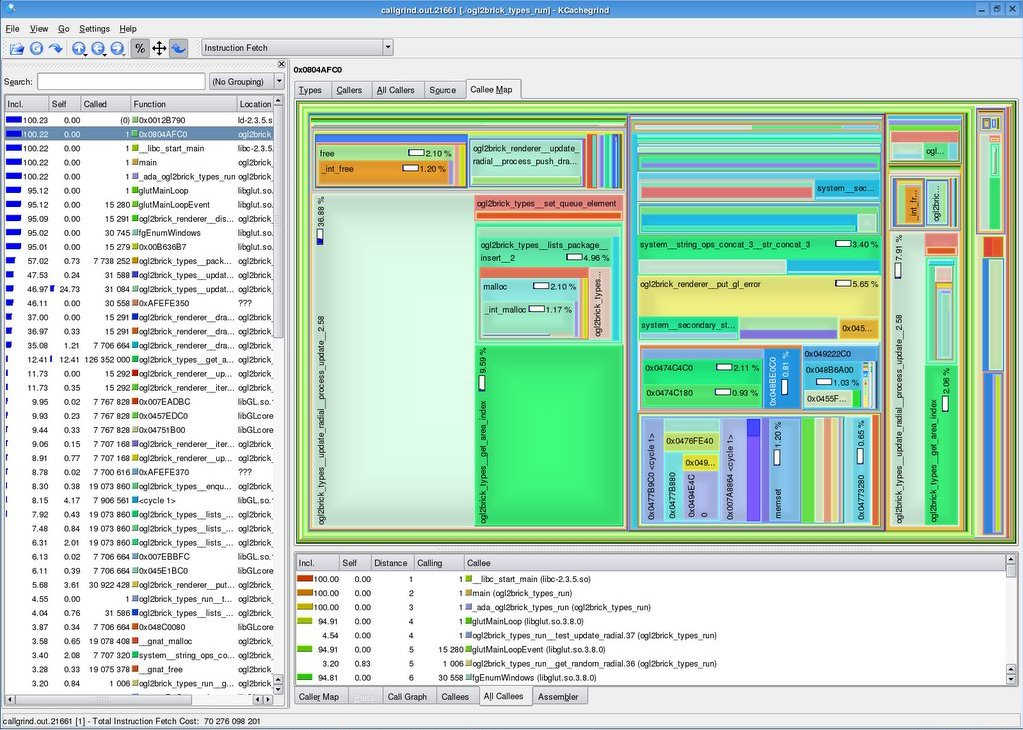
\includegraphics[width=\textwidth]{slides/sysdev-application-development/kcachegrind-screenshot.jpg}
  \end{center}
\end{frame}

\setuplabframe
{App. development and debugging}
{
  Application development
  \begin{itemize}
  \item Compile your own application with the DirectFB libraries
  \end{itemize}
  Remote debugging
  \begin{itemize}
  \item Set up remote debugging tools on the target: strace, ltrace\\
    and gdbserver.
  \item Debug a simple application running on the target using remote
    debugging
  \end{itemize}
}

\subsection{Developing on Windows}

\begin{frame}
  \frametitle{Developing on Windows!?}
  Using a GNU/Linux workstation is the easiest way to create software
  for GNU/Linux or embedded Linux
  \begin{itemize}
  \item You use the same tools and environment as all community
    developers do.  Much fewer issues you are the only one to face.
  \item You get familiar with the system.  Essential for understanding
    issues.
  \end{itemize}
  However, some developers have no choice: Windows is the only desktop
  OS allowed in their company.
\end{frame}

\begin{frame}
  \frametitle{Cygwin}
  \begin{columns}[T]
    \column{0.8\textwidth}
    \url{http://cygwin.com/}\\
    Linux (POSIX)-like environment for Windows
    \begin{itemize}
    \item 2 components:\\
      Linux API emulation layer: \code{cygwin1.dll}\\
      A collection of tools originally found in GNU/Linux
    \item Allows to compile and run many GNU/Linux programs on Windows: shells,
      compiler, http servers, X Window, GTK...
    \item Very easy to install. Can choose which tools to download and
      install.
    \item For embedded Linux system developers: makes it possible to use
      GNU toolchains (compiled for Windows) required to build Linux
      binaries (kernel, libraries or applications).
    \end{itemize}
    \column{0.2\textwidth}
    
\includegraphics[width=\textwidth]{slides/sysdev-application-development/cygwin.png}
  \end{columns}
\end{frame}

\begin{frame}
  \frametitle{Cygwin limitations}
  Cygwin is not a complete substitute for a real GNU/Linux system.
  \begin{itemize}
  \item Almost all developers work on GNU/Linux or on another Unix
    platform (typically BSD). Don't expect them to test that their
    tools build on Windows with Cygwin.
  \item The number of Cygwin users is quite small.\\
    You may be the first to face or report building issues on this
    platform for a given compiler or tool version.
  \item Cygwin is very slow.
  \end{itemize}
  So, the best solution is to run Linux inside Windows!
\end{frame}

\begin{frame}
  \frametitle{VMware}
  \begin{columns}[T]
    \column{0.8\textwidth}
    \url{http://en.wikipedia.org/wiki/VMware}
    \begin{itemize}
    \item License: proprietary
    \item Can run a GNU/Linux PC from Windows, almost at the host speed.
    \item VMware Player is now available free of charge.  Many Free
      Software system images available for download.
    \end{itemize}
    The most popular solution in the corporate world.
    \column{0.2\textwidth}
    
\includegraphics[width=\textwidth]{slides/sysdev-application-development/vmware.png}
  \end{columns}
\end{frame}

\begin{frame}
  \frametitle{VirtualBox}
  \begin{columns}[T]
    \column{0.8\textwidth}
    \url{http://virtualbox.org} from Sun Microsystems
    \begin{itemize}
    \item PC emulation solution available on both Windows and GNU/Linux
    \item 2 licenses:
      \begin{itemize}
      \item Proprietary: free of cost for personal use and evaluation.\\
        Binaries available for Windows. Full features.
      \item Open Source Edition (OSE): GPL license.\\
        Most features (except in particular USB support).\\
        No binaries released for Windows so far (but possible).
      \end{itemize}
    \item Based on QEMU's core engine. Performance similar to that of
      VMware.
    \end{itemize}
    See \url{http://en.wikipedia.org/wiki/VirtualBox}
    \column{0.2\textwidth}
    
\includegraphics[width=\textwidth]{slides/sysdev-application-development/virtualbox.png}
  \end{columns}
\end{frame}
